\documentclass[a4paper,14pt]{extarticle}

\usepackage[a4paper,top=20mm,bottom=20mm,left=30mm,right=10mm]{geometry}
\usepackage[T1,T2A]{fontenc}
\usepackage[utf8]{inputenc}
\usepackage[russian]{babel}
\usepackage{indentfirst}
\usepackage{titlesec}
\usepackage{graphicx}
\usepackage{listings}

\renewcommand{\baselinestretch}{1.3}
\titleformat{\section}{\normalsize\bfseries}{\thesection}{1em}{}
\titleformat{\subsection}{\normalsize\bfseries}{\thesection}{1em}{}
\setlength{\parindent}{12.5mm}

\begin{document}
	
	\newpage\thispagestyle{empty}
	\begin{center}
		\MakeUppercase{
			Министерство науки и высшего образования Российской Федерации\\
			Федеральное государственное бюджетное образовательное учреждение высшего образования\\
			<<Вятский Государственный Университет>>\\
		}
		Институт математики и информационных систем\\
		Факультет автоматики и вычислительной техники\\
		Кафедра электронных вычислительных машин
	\end{center}
	\vfill
	
	\begin{center}
		Отчет по лабораторной работе №5\\
		по дисциплине\\
		<<Информатика>>\\
		<<Представление вещественных чисел в формате с плавающей точкой>>
	\end{center}
	\vfill
	
	\noindent
	\begin{tabular}{ll}
		Выполнил студент гр. ИВТб-1301-05-00 \hspace{5mm} &
		\rule[-1mm]{25mm}{0.10mm}\,/Макаров С.А./\\
		
		Руководитель доцент кафедры ЭВМ & \rule[-1mm]{25mm}{0.10mm}\,/Коржавина А.С./\\
	\end{tabular}
	
	\vfill
	\begin{center}
		Киров 2024
	\end{center}
	
	\newpage
	\section*{Цель}
	Цель лабораторной работы: закрепить на практике знания форматах представления числовой информации. Написать программы, решающие описанные ниже задачи.
	
	\section*{Задание}
	\begin{enumerate}
		\item Представить число в формате с плавающей точкой в n-разрядной сетке. Формат аналогичен IEEE 754. На входе: вещественное число в десятичной системе счисления, разрядность сетки, число разрядов мантиссы. На выходе: строка, отображающая введенное число в формате с плавающей точкой.
		
		\item Представить число в формате с плавающей точкой в n-разрядной сетке. Нормализация мантиссы дробная, формат с порядком, последовательность отображения – знак, мантисса, порядок. На входе: вещественное число в десятичной системе счисления, разрядность сетки, число разрядов мантиссы. На выходе: строка, отображающая введенное число в формате с плавающей точкой.
		
		\item Представить число в формате с плавающей точкой в n-разрядной сетке. Нормализация мантиссы дробная, формат с характеристикой, последовательность отображения – знак, мантисса, характеристика. На входе: вещественное число в десятичной системе счисления, разрядность сетки, число разрядов мантиссы. На выходе: строка, отображающая введенное число в формате с плавающей точкой. 
	\end{enumerate}
	
	\newpage
	\section*{Решение}
	Для решения представленных задач создадим подпрограмму побитового вывода десятичного числа, представленная на рисунке 1. Исходный код подпрограммы на языке C представлен в приложении А.
	
	\begin{figure}[h]
		\centering
		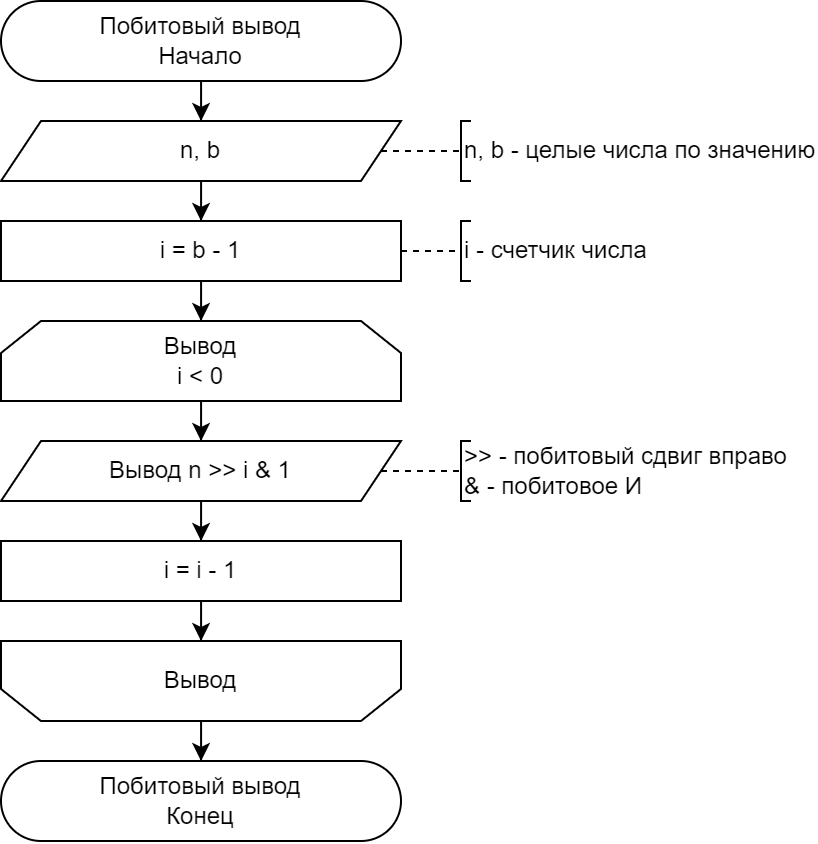
\includegraphics[width=0.65\linewidth]{schemes/s-p}
	\end{figure}
	\begin{center}
		Рисунок 1 – Схема алгоритма подпрограммы <<Побитовый вывод>>
	\end{center}
	
	\pagebreak
	\subsection*{Задание 1}
	Схема алгоритма для решения предлагаемой задачи представлена на рисунке 2. Исходный код на языке C представлен в приложении А.
	\begin{figure}[h]
		\centering
		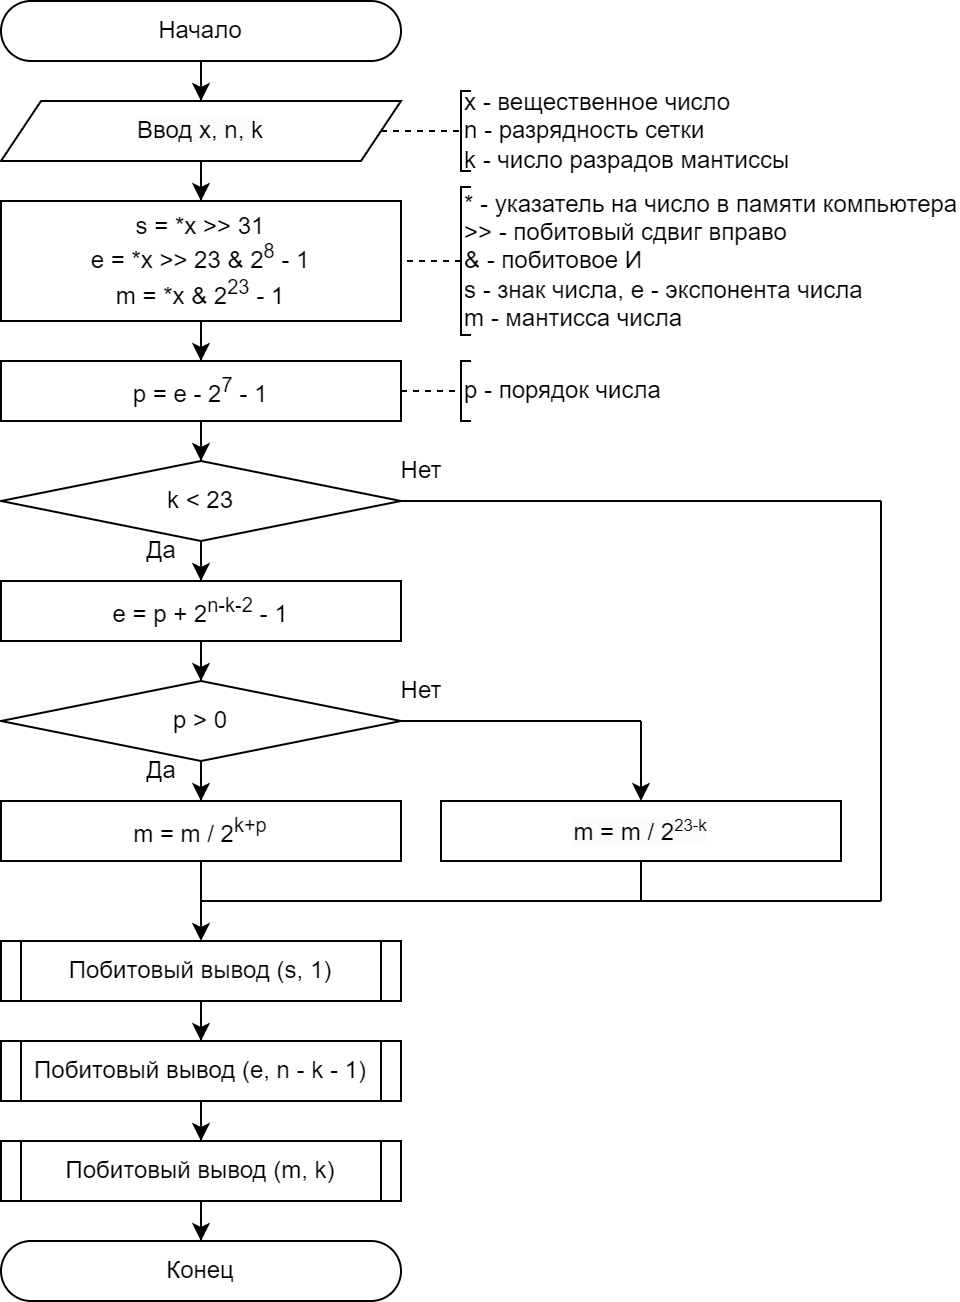
\includegraphics[width=0.65\linewidth]{schemes/s-1}
	\end{figure}
	\begin{center}
		Рисунок 2 – Схема алгоритма задания 1
	\end{center}
	
	\pagebreak
	\subsection*{Задание 2}
	Схема алгоритма для решения предлагаемой задачи представлена на рисунке 3. Исходный код на языке C представлен в приложении А.
	\begin{figure}[h]
		\centering
		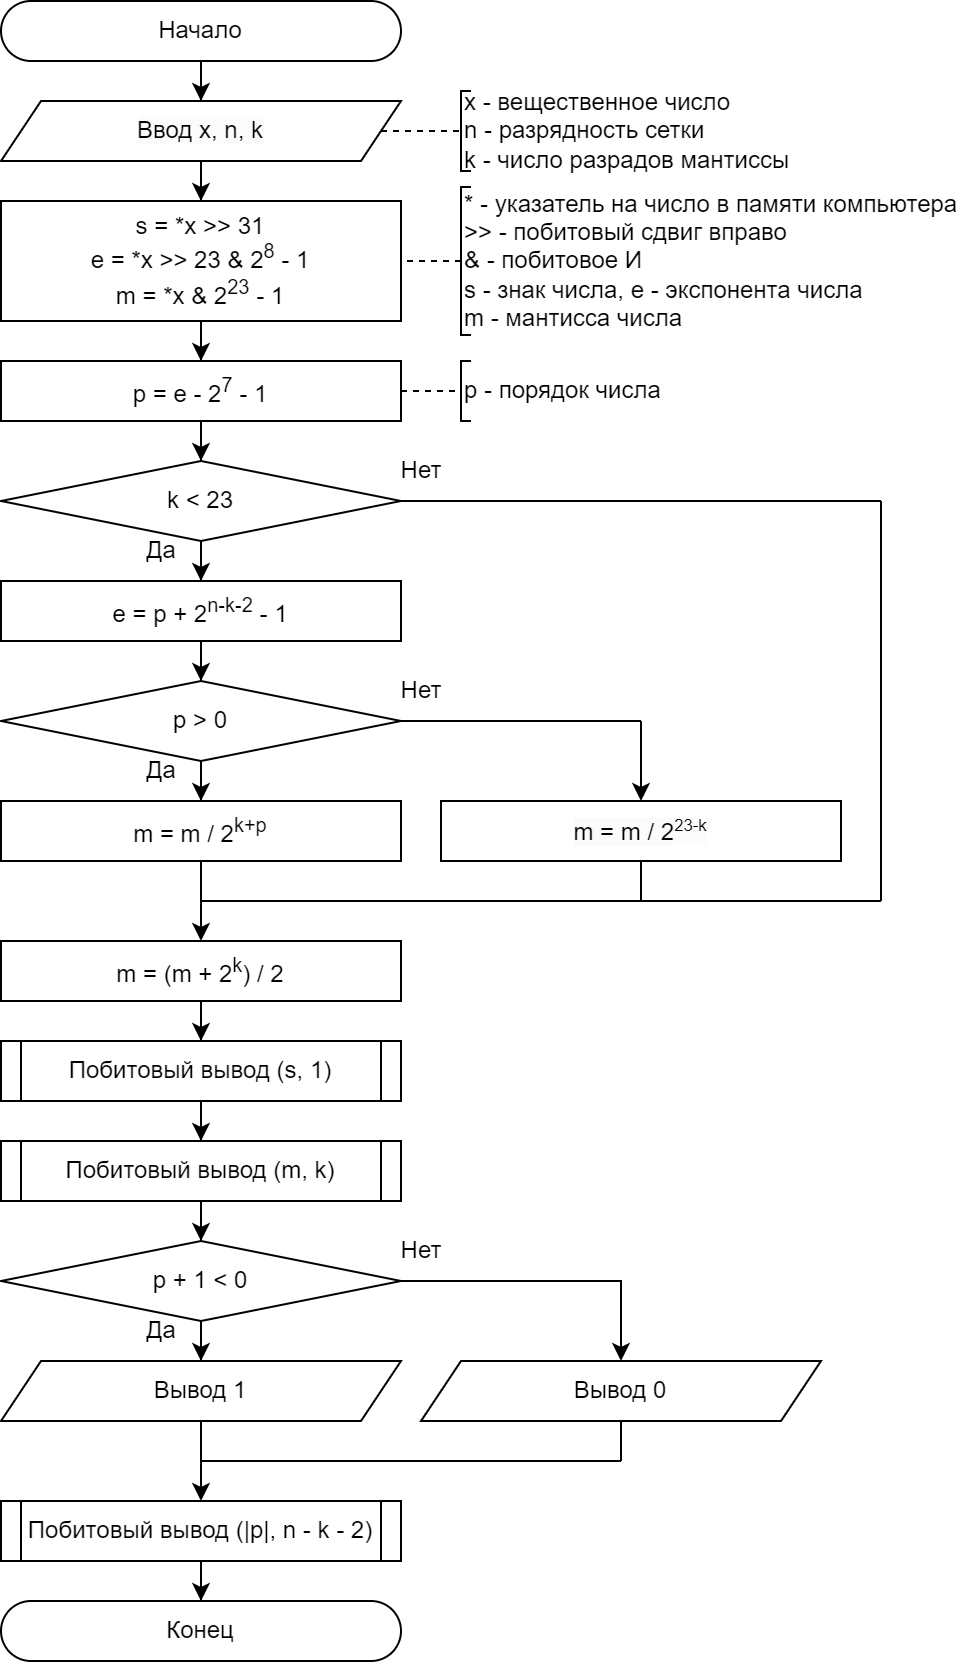
\includegraphics[width=0.65\linewidth]{schemes/s-2}
	\end{figure}
	\begin{center}
		Рисунок 3 – Схема алгоритма задания 2
	\end{center}
	
	\pagebreak
	\subsection*{Задание 3}
	Схема алгоритма для решения предлагаемой задачи представлена на рисунке 4. Исходный код на языке C представлен в приложении А.
	\begin{figure}[h]
		\centering
		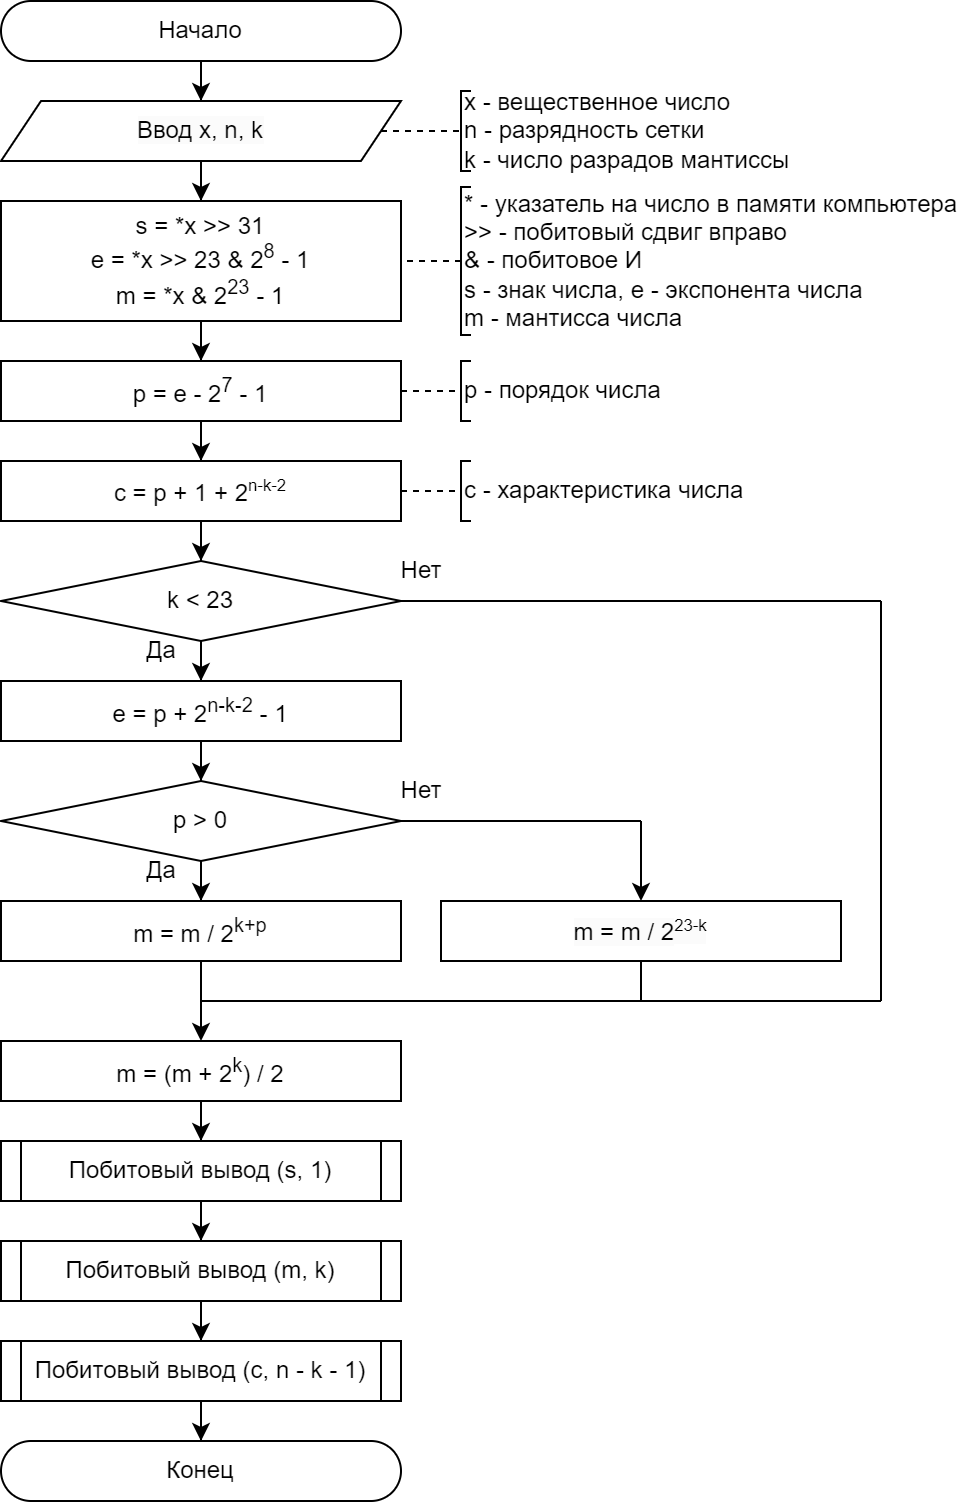
\includegraphics[width=0.6\linewidth]{schemes/s-3}
	\end{figure}
	\begin{center}
		Рисунок 4 – Схема алгоритма задания 3
	\end{center}
	
	\section*{Вывод}
	В ходе выполнения лабораторной работы удалось закрепить на практике знания использования формата представления числовой информации. Были реализованы программы вывода числа в форматах IEEE-754, порядка, характеристики, написанных на языке C.
	
	\newpage
	\section*{Приложение А}
	\begin{lstlisting}[tabsize=2,basicstyle=\ttfamily]
#include <stdio.h>
#include <math.h>

void print_bin(int n, int b) {
	for (int i = b - 1; i >= 0; i--) {
		printf("%d", n >> i & 1);
	}
}

int main() {
	float x; int n, k;
	scanf("%f %d %d", &x, &n, &k);
	
	int* d = (int*) & x;
	int s = *d >> 31;
	int e = *d >> 23 & (int)pow(2, 8) - 1;
	int m = *d & (int)pow(2, 23) - 1;
	int p = e - (pow(2, 7) - 1);
	int c = p + 1 + pow(2, n - k - 2);
	e = p + (pow(2, n - k - 2) - 1);
	
	if (k < 23) {
		if (p > 0) {
			m = m / pow(2, k + p);
		} else {
			m = m / pow(2, 23 - k);
		}
	}
	\end{lstlisting}

	\pagebreak
	\section*{Продолжение приложения А}
	\begin{lstlisting}[tabsize=2,basicstyle=\ttfamily]
	print_bin(s, 1);
	print_bin(e, n - k - 1);
	print_bin(m, k);
	printf("\n");
	
	m = (m + pow(2, k)) / 2;
	
	print_bin(s, 1);
	print_bin(m, k);
	printf("%d", p + 1 < 0 ? 1 : 0);
	print_bin(abs(p + 1), n - k - 2);
	printf("\n");
	
	print_bin(s, 1);
	print_bin(m, k);
	print_bin(c, n - k - 1);
	printf("\n");
	
	return 0;
}
	\end{lstlisting}
	
\end{document}